\documentclass[tikz,border=10pt]{standalone}
\begin{document}
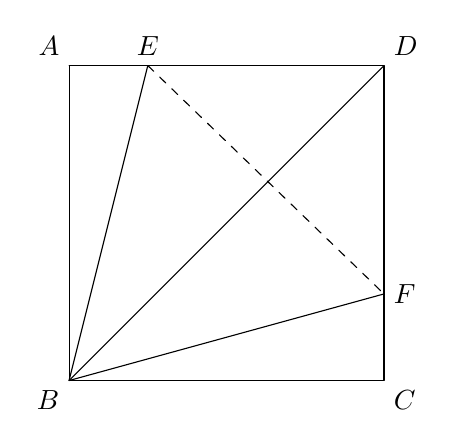
\begin{tikzpicture}[line cap=round,line join=round,scale=1]

\coordinate (A) at (0,4);
\coordinate (B) at (0,0);
\coordinate (C) at (4,0);
\coordinate (D) at (4,4);
\coordinate (E) at (1,4);
\coordinate (F) at (4,1.1);

\draw (A) -- (B) -- (C) -- (D) -- (A);
\draw (B) -- (E);
\draw (B) -- (D);
\draw (B) -- (F);
\draw[dashed] (E) -- (F);

\node[above left] at (A) {$A$};
\node[below left] at (B) {$B$};
\node[below right] at (C) {$C$};
\node[above right] at (D) {$D$};
\node[above] at (E) {$E$};
\node[right] at (F) {$F$};

\end{tikzpicture}
\end{document}
